%!TEX root = ../thesis.tex

%invariant enviroment
\newenvironment{invariants}{%
  \refstepcounter{thrm}%
  \paragraph{Invariants~\theprop}%
  \renewcommand*{\theenumi}{\theprop\,(I\arabic{enumi})}%
  \renewcommand*{\labelenumi}{(I\arabic{enumi})}%
  \enumerate
}{%
  \endenumerate
}

\section{Algorithms}
\label{s:algo}
Kant and He \cite{Kant1997} were the first to design algorithms that determine a regular edge labeling.

Fusy \cite{Fusy2006} recently developed a different algorithm computing a specific regular edge labeling using a method shrinking a sweepcycle while coloring the outside in accordance with a regular edge labeling.\footnote{The specific regular edge labeling Fusy obtained was the minimal element of the distributive lattice of regular edge labellings.}

All algorithms in this section will have the same core (based on \cite{Fusy2006}). Consisting of shrinking a sweepcycle by so called \emph{valid} paths.\footnote{In Fusy's work he calls these \emph{eligible paths}} But will differ in which valid paths they choose (if there are multiple).

We will start this section with some notation and preliminaries in Subsection \ref{ss:not}. Then we will state the core algorithm and show that it always computes a regular edge labeling in Subsection \ref{ss:core}. Afterwards we show in Subsections \ref{ss:minimal}, \ref{ss:blue} and Section \ref{s:red} how one can adapt the choice of the valid paths to obtain regular edge labellings with certain properties. Namely a the minimal element of the distributive lattices of regular edge labellings and regular edge labeling corresponding to horizontal and vertical rectangular duals.


\subsection{Notation and Preliminaries}
\label{ss:not}
\begin{defi}[Interior path]
We call a path $P$ an internal path of a cycle $C$ if all vertices except the first and last one are in the interior of $C$ and it connects two distinct vertices of $C$
\end{defi}

We will use a script $\C$ to indicate the current sweep cycle.
We will repeatedly only consider the path $\cpath$. In that case we will always order it from $\pW$ to $\pE$. That these edges are always in $\C$ is a result of Invariant \ref{i:SWandSE}.

We will let $\P$ denote a interior path. Given such a path of $k$ vertices we will index it's nodes by $p_1, \ldots, p_k$ in such a way that $p_1$ is closer to $\pW$ then $p_k$ is (and thus that $p_k$ is closer to $\pE$ then $p_1$ is).

Then $p_1$ and $p_k$ indicate the two unique vertices of the walk that are also part of the cycle. We will then let $\restC{\P}$ denote the part of $\cpath$ that is between $p_1$ and $p_k$ (including). $\C_\P$ will denote the cycle we get when we paste $\restC{\P}$ and $\P$.



\subsection{Core}
\label{ss:core}

The algorithm will always maintain the following three invariants

\begin{invariants}
  \itemsep=-4pt

\item \label{i:SWandSE} The cycle $\C$ contains the two edges $\pS \pW$ and $\pS \pE$.
\item \label{i:noChords} $\cpath$ has no chords
\item \label{i:last} All inner edges of $T$ outside of $\C$ are colored and oriented in such that the inner vertex condition holds. %TODO what is the inner vertex condition
\fxerror{We need to add a partial inner vertex condition}
\end{invariants}

A cycle satisfying these three invariants will have the same general shape as in figure \ref{fig:invCycle}. We note that the cycle has at least $4$ vertices because otherwise a separating triangle is created.

\begin{figure}[h!]
\centering
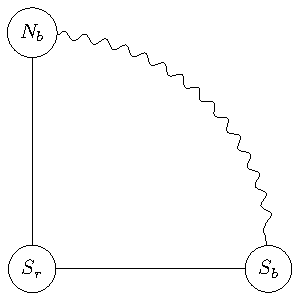
\includegraphics{algo/img/invCycle}

\caption{An example of a cycle $\C$ satisfying the invariants
    \label{fig:invCycle}}
\end{figure}

It is also nice to note that the union of the cycle and it's interior form a triangulation of the $n$-gon since it is a induced subgraph of a triangulation of the $4$-gon.


\subsubsection{Valid paths}

\begin{defi}[valid path]
We call an internal path $\P$ from $w_1$ to $w_k$ valid if
\begin{enumerate}
 \renewcommand*{\labelenumi}{(E\arabic{enumi})}%
 \renewcommand*{\theenumi}{(E\arabic{enumi})}%


\item Neither $p_1$ or $p_k$ is $\pS$
\label{e:noS}

\item The paths $\P$ and $\restC \P$ both have more than 1 edge \footnote{i.e. both have an interior vertex}
\label{e:longBorders}

\item Every interior edge of $\C_\P$ connects a vertex of $\P\setminus{\braces{p_1,p_k}}$ and $\restC \P \setminus{\braces{p_1,p_k}}$. In particular $\C_\P$ is a non-separating cycle.
\label{e:crossingEdges}

\item The path $\C'\sm{\pS}$, where $\C'$ is obtained by replacing $\restC \P$ by $\P$ in $\C$, is chordfree.
\label{e:noNewChord}

\end{enumerate}
\end{defi}

We note that \ref{e:crossingEdges} and \ref{e:noNewChord} partially overlap. \ref{e:crossingEdges} already implies that there can't be chords on the left of $\cpath$.


\begin{remark}
``Shrinking'' the cycle with an valid path will keep all the invariants true.
\end{remark}
\fxwarning[inline, nomargin]{We haven't proven this yet}

We will show the following proposition.



\begin{thrm}[Existence of a eligible path]
\label{th:eligExistence}
When the algorithm's invariant (\ref{i:SWandSE} - \ref{i:last}) are satisfied and the cycle $\C$ is separating then there exist a \emph{eligible} internal path.
\end{thrm}
\fxerror[inline, nomargin]{As outlined in last meeting this proof is not complete as is, it has been moved to the appendix. We are stuck on the part where we need to find a path satisfying E4. We might proof this from red algo.}



\subsection{Minimum distributive lattice element}
\label{ss:minimal}
We get this when we take the ``leftmost'' eligible path. As is outlined in \cite{Fusy2006}
\fxnote{Expand this subsection}

\renewcommand{\F}{\scr F}
\subsection{Horizontal one-sides}
\label{ss:blue}
\fxerror{Define what we mean with \emph{cycle border} and \emph{face border}}

As an exercise one could try to adapt Fusy's algorithm to generate horizontally one-sided layouts directly, without doing flips in the distributive lattice. It turns out that this is not that difficult.

Since the horizontal segments correspond to faces in the blue bipolar orientation we want that one of the two borders of the face has a length of at most two. Since every valid path which we update the cycle with splits off one face in the blue bipolar orientation it is easy to control this property.

\begin{thrm}
\label{th:blueelig}
In the update of the algorithm there is always an eligible path $\P$ available such that either $\P$ or $\restC{\P}$ is of length $2$.
\end{thrm}

In order to proof this theorem we will first show the following lemma.

\begin{lemma}
\label{lem:bluealgo}
If $\P$ is an eligible path giving raise to a cycle $\C_P$ of which both borders have length of at least $3$. Then there exist an eligible path $\P'$ such that the path border and cycle border of its cycle $\C_{\P'}$ are both at least $1$ shorter than those of $\C_\P$.
\end{lemma}

\fxnote{Revisit notation after writing section on oriented REL}
\begin{proof}
In this proof we will frequently use property \ref{e:crossingEdges} of a valid path, we won't mention it every time we use it.

We denote the source by $s$ and the sink by $t$. We also assign names$a, b$ and $x, y$ to the first two vertices on both borders, see Figure \ref{fig:bluealgo:notation}. Since every interior face of $G$ is a triangle $ax$ is an edge. Now we distinguish two cases, either $ay$ is an edge (case 1) or $bx$ is an edge (case 2). They can't both be an edge at the same time due to planarity, neither can it happen that both of them are not an edge since then the face containing the path $baxy$ is at least of degree $4$.

In the first case $a$ may be connected to more vertices on the path border, however there is a last one, say $z$. And this vertex is then also connected to $b$, otherwise it would not be the last one. Now we can provide an shorter eligible path $\P'$. We start at $a$ go to $z$ and from there we follow the old path $\P$ to $t$.  See figure \ref{fig:bluealgo:case1}. It is easy to see that all four properties of an eligible path hold for $\P'$.
\begin{comment}
By construction $\P'$ satisfies \ref{e:noS} and \ref{e:internalVertices}. While the interior of $\C_{\P'}$ is a subset of that $\C_\P$%TODO this is again an eligible path
\end{comment}

In the second case $x$ may be connected to more vertices along the cycle border, however there is a last one, say $c$. And this vertex is then also connected to $y$, otherwise it would not be the last one. Now we can provide an shorter eligible path $\P' = sxz$.   See figure \ref{fig:bluealgo:case2}. It is straightforward to see that all four properties of an eligible path hold for $\P'$. %TODO this is again an eligible path
\end{proof}

\begin{figure}[ht]
    \centering
    \begin{subfigure}[b]{0.45\textwidth}
        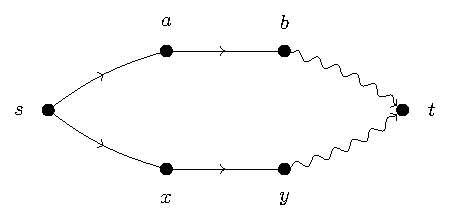
\includegraphics[width=\textwidth]{algo/img/blue/setting}
        \caption{The setting}
        \label{fig:bluealgo:notation}
    \end{subfigure}

    \begin{subfigure}[b]{0.45\textwidth}
        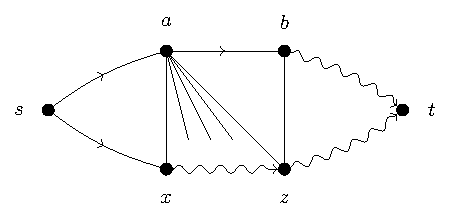
\includegraphics[width=\textwidth]{algo/img/blue/case1}
        \caption{Case 1}
        \label{fig:bluealgo:case1}
    \end{subfigure}
    ~
    \begin{subfigure}[b]{0.45\textwidth}
        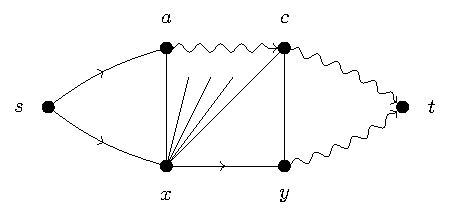
\includegraphics[width=\textwidth]{algo/img/blue/case2}
        \caption{Case 2}
        \label{fig:bluealgo:case2}
    \end{subfigure}

    	\caption{}
\end{figure}

\begin{proof}[Proof of Theorem \ref{th:blueelig}]
By Theorem \ref{th:eligExistence} we know there is a eligible path $\P$. If one of the borders of $\C_\P$ is of length $2$ or less we are done. If this path gives raise to a face $\C_\P$ with both borders are both of length at least $3$ we can repeatedly apply Lemma \ref{lem:bluealgo} until at least one of the borders is of length at most $2$.
\end{proof}

If we in every update of the algorithm take the paths from Theorem  \ref{th:blueelig} we end up with the correct faces in the blue bipolar orientation and hence a horizontally one sided rectangular dual.
